\documentclass{article}
\usepackage[affil-it]{authblk}
\usepackage{graphicx}
\usepackage[space]{grffile}
\usepackage{latexsym}
\usepackage{amsfonts,amsmath,amssymb}
\usepackage{url}
\usepackage[utf8]{inputenc}
\usepackage{hyperref}
\hypersetup{colorlinks=false,pdfborder={0 0 0}}
\usepackage{textcomp}
\usepackage{longtable}
\usepackage{multirow,booktabs}
\usepackage{natbib}
\bibliographystyle{plainnat}
\usepackage{lineno}
\usepackage{setspace} 
\doublespacing

% Text layout
\topmargin 0.0cm
\oddsidemargin 0.5cm
\evensidemargin 0.5cm
\textwidth 16cm 
\textheight 21cm

\begin{document}

\title{Supplementary material for ``The genetic backburn: a management tool for halting invasions."}

\author{Ben L. Phillips}
\affil{School of Biosciences, University of Melbourne}

  
\author{Rick Shine}
\affil{School of Biological Sciences, University of Sydney}
  
\author{Reid Tingley}
\affil{School of Biosciences, University of Melbourne}
  


\date{\today}

\bibliographystyle{plain}

\maketitle 



\section{Long-distance dispersal}

As described in the main methods, long-distance dispersal was implemented by changing the shape parameter, $v$, of the scaled t-distribution.  We chose values of $v$ that gave excess kurtosis values of 1, 2, and 3.  These excess kurtosis values correspond to increasing probability of long-distance dispersal by individuals in the model.  We ran the values of $v$ with the default values for other parameters (in particular, with $k=0.2$).

Increasing the probability of long distance dispersal led directly to thinner barriers being less effective.  As a consequence, a barrier of width ten units was almost always breached, and so we don't show those results.  Instead, we show the results for barriers of width 15, and 30 units.  Under Gaussian dispersal (excess kurtosis = 0), these barrier widths span the range from a barrier that is always effective, through to a barrier that is dramatically improved by a genetic backburn.  Increasing the kurtosis of the kernel caused both barriers to become generally less effective, but it also led to a weaker effect of genetic backburning (\emph{cf.} backburn extent 0, to extents \textgreater 0).

 \begin{figure}[h!]
\begin{center}
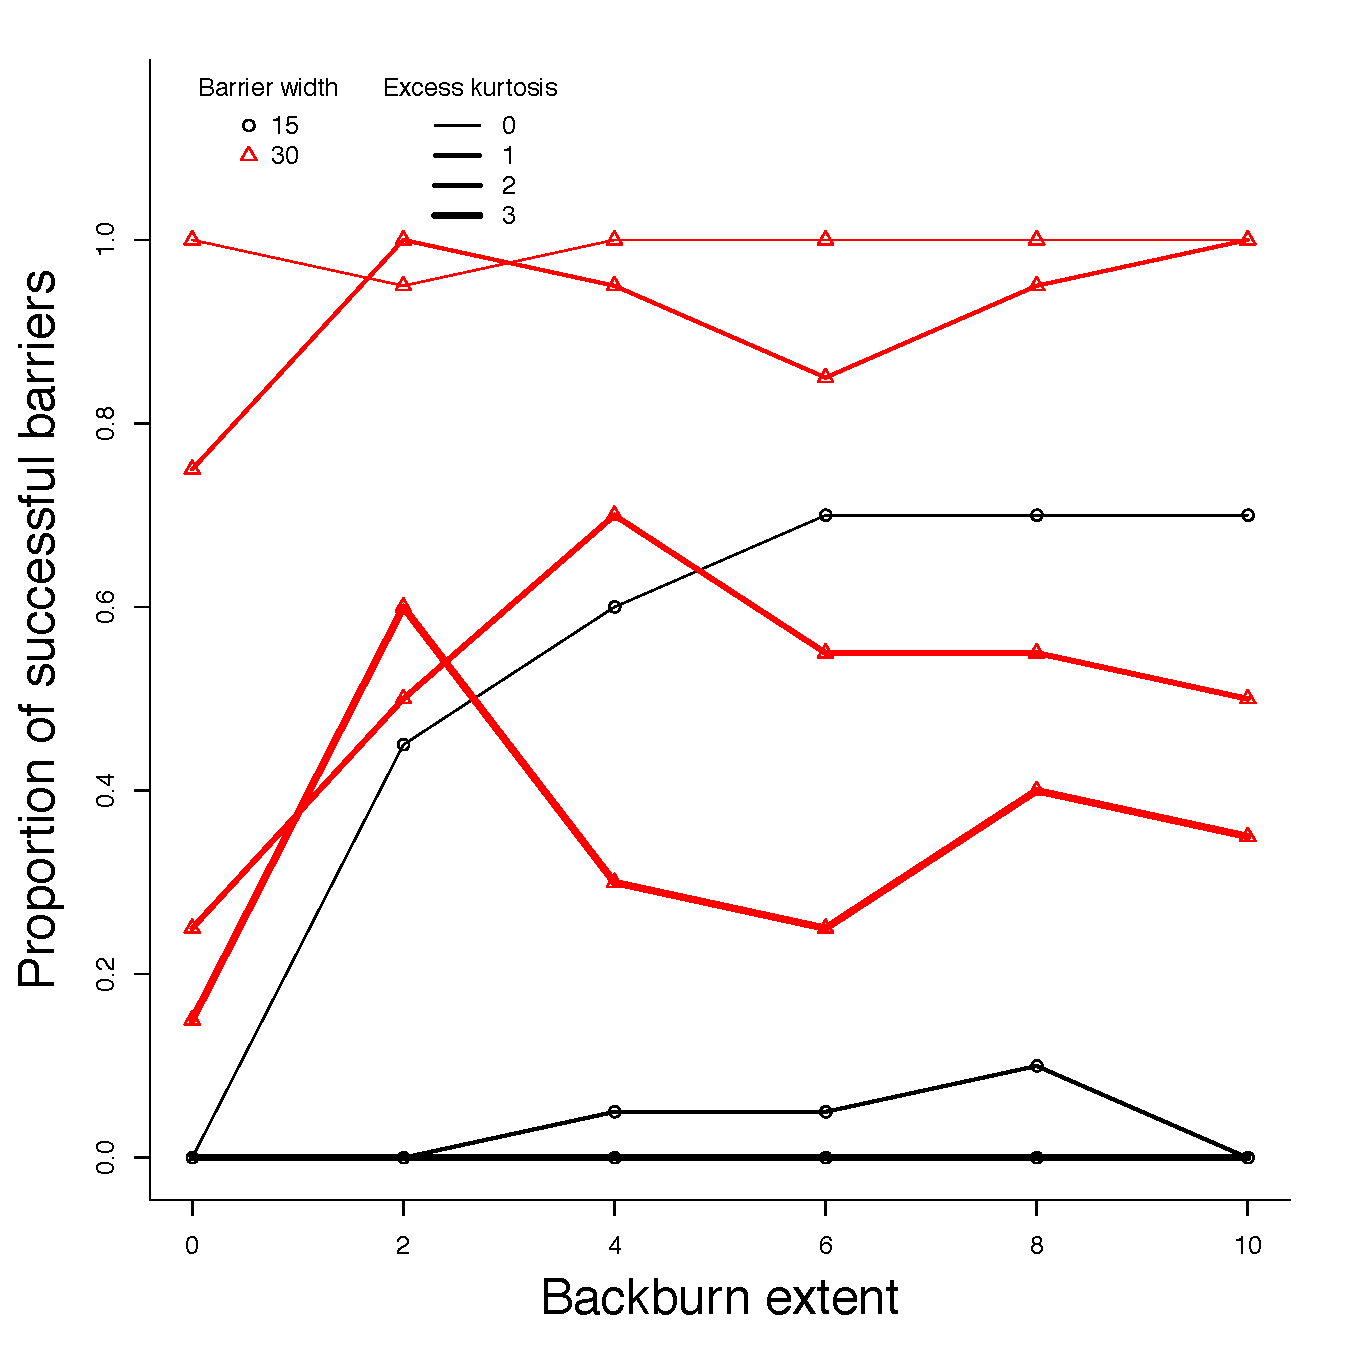
\includegraphics[width=0.7\columnwidth]{BarSimsVarv.pdf}
\caption{\label{fig:varv}
The strength of a barrier can be influenced by a genetic backburn.  Here we show two barrier sizes (widths = 15 and 30 units), and the proportion (of 20 simulations) in which, over 50 generations, the barrier stops the invasion.  In almost all cases where improvement was possible, the strength of the barrier was improved by a genetic backburn.  This improvement in barrier strength was, however, dependent on the degree of long-distance dispersal (increasing long-distance dispersal given by increasing values for excess kurtosis).  Increasing long-distance dispersal (excess kurtosis \textgreater 0) also generally made barriers weaker compared with scenarios where long-distance dispersal was absent (excess kurtosis = 0).}
\end{center}
\end{figure}



\end{document}